\section{Présentation du contexte du projet}
    \subsection{\company{}}
        \subsubsection{Qui est \texorpdfstring{\gls{mdi}}{MDI}?}
            \company{}\cite{mdi_site}, un des leaders mondiaux de la télématique, est une entreprise
            française spécialisée dans les systèmes embarqués pour l'automobile.
            L’entreprise dont le siège est situé en région parisienne (à Villejuif) a depuis à peu près
            15 ans, conçu et développé des boîtiers connectés aux véhicules par port OBD (On
            Board Diagnostics).\\
            Actuellement, \gls{mdi} comprend une cinquantaine d’employés répartis dans plusieurs
            pays dont la France, les États-Unis  Irlande. Avec un chiffre d’affaire de
            plusieurs dizaines de millions d’euros et plus d’un million de boîtiers déployés dans le
            monde.\\


            ((((((((((((((((((((((((((((((figure : carte du monde montrant les pays où se trouvent MdI ( fr , USA , AS ) et les 
            pays ou les OBD sont déployés ( les clients:  ( l’Afrique du sud,Autriche, Belgique, Bulgarie, Croatie, Chyprés, République Tchèque, Danemark, Estonie, ETats unies, Finlande, France, Allemagne, Grèce, Hongrie, Ireland, Italie, Lettonie, Lituanie, Luxembourg, Malte, Pays bas, Pologne, Portugal, Romanie, Slovaquie, Slovénie, Espagne, Suède, Suisse, Grande Bretagne))))))))))))))))))))))))))))))))
            \begin{figure}[ht]
                \centering
                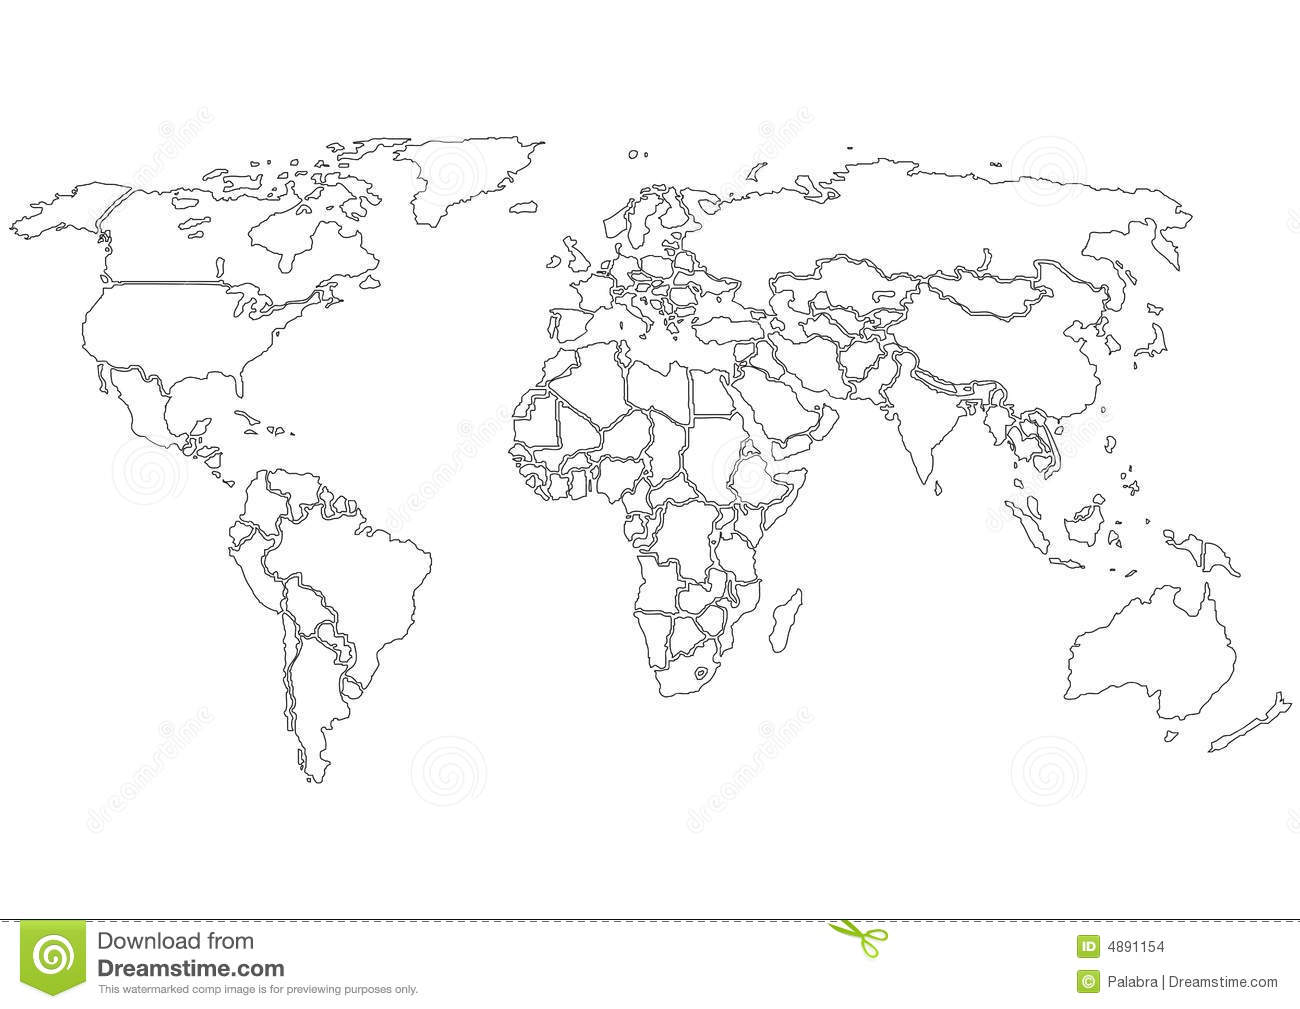
\includegraphics[scale=1]{\images/cartemonde1.jpg}
                \caption{Les pays où circulent des véhicules ayant des OBD déployés }
            \end{figure}


            
            Les clients de Mobile Devices Ingénierie sont ainsi réparties partout dans l'Europe et les États Unies. 
            En effet, ils occupent différents secteurs d’activités tels que :\\
            \begin{itemize}
                \renewcommand{\labelitemi}{$\bullet$}
                \item Des applications embarquées de gestion de flottes de taxis 
                \item Des compagnies d’assurances 
                \item Des compagnies de navigation et d'info trafic 
                \item Des revendeurs qui adaptent les produits MDI à leurs services et qui disposent d’un accès à certains marchés de par leur histoire ou leur image de marque.
            \end{itemize}


        \subsubsection{Domaine d'activité et Stratégie }
            L’objectif de l'entreprise est de devenir le leader mondial pour l'acquisition, le
            traitement, l'enrichissement et l’échange des données techniques de véhicules
            connectés.\\

            Mobile Devices Ingénierie a pour secteur d’activité la télématique embarquée pour l'automobile. 
            Concrètement, cela consiste à proposer des solutions techniques permettant l'échange d'informations 
            entre un ou plusieurs systèmes de gestion centralisés et une flotte de véhicule qui y est rattachée 
            et connectée en temps réel.
            Ces informations sont ensuite récupérées en temps réel et peuvent être envoyées 
            vers les serveurs de l’entreprise ou des clients. \\

            \begin{figure}[ht]
                \centering
                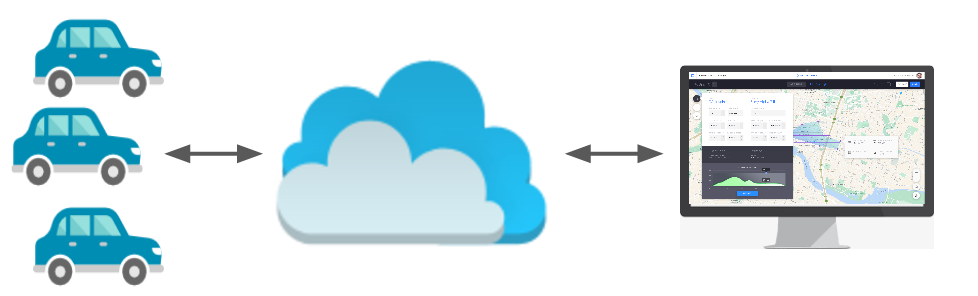
\includegraphics[scale=0.4]{\images/carcloud.png}
                \caption{Schema représentant le circuit des données remontés  }
            \end{figure}
            
            L’activité principale de Mobile Devices Ingénierie se résume à la mise en place de solutions techniques 
            afin d’effectuer le suivi de véhicules et la gestion de flottes. Les produits de l'entreprise permettent 
            de récupérer des données telles que la vitesse, la consommation, le type de conduite et même de prévenir 
            des accidents.
            Ces mêmes données permettent ensuite, par exemple pour certaines entreprises, d’étudier la conduite 
            des véhicules et leurs différents paramètres comme suivre un déplacement et/ou quantifier la consommation 
            dans le cas d’une gestion de flotte. \\
            Ces données peuvent aussi servir à étudier le type de conduite dans le cas d’une compagnie d’assurance. 
            La société compte aussi d'autres activités comme la commercialisation des boîtiers pouvant offrir l’aide 
            à la navigation servant par exemple aux Taxis.
            Les entreprises clientes peuvent aussi reprogrammer une partie de leurs boîtiers afin de récupérer des données 
            spécifiques et les transférer vers des serveurs distants. \\

            Par la nature même de l’activité, l’entreprise apporte à ses clients des solutions
            innovantes permettant de concilier le développement économique et la préservation de l’environnement.
            En effet, ses solutions permettent de mettre en œuvre le contrôle
            de baisse de la consommation énergétique, de l’empreinte carbone des
            véhicules et du risque environnemental associé.\\[0.3cm]
            Dans le cadre de son développement durable, la protection de l’environnement est une
            préoccupation fondamentale pour \gls{mdi}. L’éthique, l’équité et la diversité sont des
            facteurs de progrès qui contribuent à améliorer les résultats économiques ainsi que le
            climat social, éléments clefs d’un développement durable pour \company{}.

        \subsubsection{Organisation et produits}
        L’entreprise suit un schéma d’organisation hiérarchique fonctionnelle composée d’une division classique du 
        travail par fonctions. Elle est constituée d’un dirigeant et ensuite d’une équipe de collaborateurs ayant 
        différentes fonctions : commerciales, comptables, financières, ressources humaines, productions, etc. 
           Quant au côté technique, \gls{mdi} articule plusieurs types d'équipes: \\
            \begin{itemize}
                \renewcommand{\labelitemi}{$\bullet$}
                \item L’équipe \textbf{Production} en charge de la production et la livraison des produits
                \item L’équipe \textbf{Core} en charge de « Morpheus » (le système d’exploitation applicatif du boîtier)
                \item L’équipe \textbf{Système} en charge du système d'exploitation linux
                \item L’équipe \textbf{Pre-Sales} en charge du support clients et accompagement des commerciaux
                \item L’équipe \textbf{Serveur} en charge du cloud, au sein de laquelle j'ai effectué mon stage
            \end{itemize} 
            
            \vspace{0.5cm}

        Ces équipes travaillent sur différents projets autour des produits hardwares et softwares: 
            \begin{table}[h!]
                \centering
                \begin{tabular}{|p{5cm}|p{5cm}|}
                    \hline   Les produits Hardwares & Les produits Softwares \\
                    \hline
                    \begin{itemize}
                        \renewcommand{\labelitemi}{$\bullet$}
                        \item munic.io
                        \item municMax
                        \item \gls{obd} Dongle
                    \end{itemize} 
                   & 
                    \begin{itemize}
                        \renewcommand{\labelitemi}{$\bullet$}
                        \item Morpheus OS
                        \item CloudConnect
                        \item CloudNext
                    \end{itemize}\\
                    \hline 
                \end{tabular}
                \caption{Tableau des produits MDI}
                \label{table:1}
            \end{table} \\

            \vspace{0.3cm}

            Les produits Hardwares sont intégrés dans les véhicules et récoltent des informations sur 
            la vitesse, la position, le niveau de carburant, la pression des pneus, etc..  à un instant t donnée.
            En général nous appelons ces produits hardwares “les boîtiers” qui doivent être intégrés dans 
            les véhicules et déployés  dans le système cloud. \\ [0.1cm]
            Quant aux produits Softwares, il y a le Morpheus OS qui présente le système d'exploitations des boîtiers. 
            D'autre part,les clouds CloudConnect et CloudNExt qui offrent un ensemble de services aux clients 
            et qui sont développés et maintenus par l'équipe Serveur. On détaillera plus sur ces deux produits dans le prochain chapitre. 
       
        \subsection{Présentation du projet}
        \subsubsection{Contexte du projet}
            Mon sujet principal de stage est la conception et développement du nouveau composant du Cloud. Ce composant représente 
            le point d'entrée des données au cloud. Il assure la communication entre le cloud et les boîtiers. 
            Le composant actuel porte le nom de \gls{BS} - acronyme de Binary Server. Il est intégré seulement dans CloudConnect.
            \begin{figure}[ht]
                \centering
                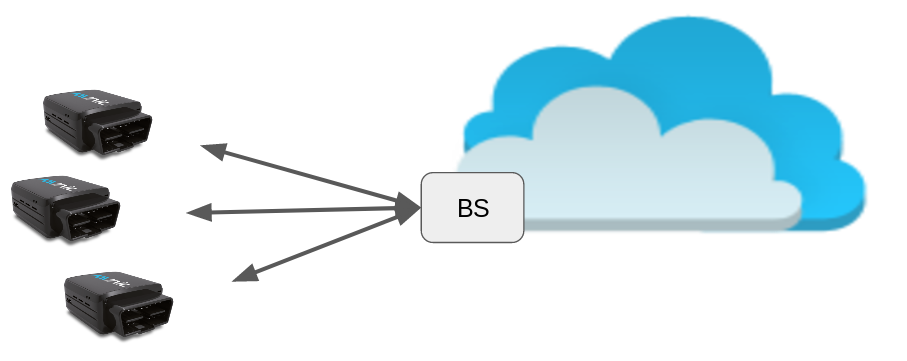
\includegraphics[scale=0.3]{\images/bs.png}
                \caption{BS le seul point d'entrée des clouds }
            \end{figure}
           
        \subsubsection{Problématique}
            Plusieurs facteurs  rendent le développement d'un noouevau composant cloud une nécessité. 
            \\Dans l’architecture actuelle, les deux cloud sont totalement indépendants mais ils reçoivent les données 
            de la même source \gls{BS} malgré la différence entre les deux formats de messages. \\ 

            D'autre part , pour une raison commercial, le nouveau protocole migre d'un protocole fait maison vers un protocole standardisé. \\
            Un standard permet de bénéficier des librairies existantes sur le marché et donc de gagner en temps d'intégration puisque 
            il' n y aura pas le besoin de faire du développement à zéro.
            MQTT n'étant pas propriétaire, les partenaires ou clients savent également comment celui-ci est conçu. Ce qui n'est pas le cas 
            pour \gls{mdi21} \- le protocole actuel fait maison \-  donc cela permet de rassurer le client. 
            Le "standard MQTT" permets également de laisser d'autres boîtiers se connecter à notre plate-forme plus facilement 
            plutôt que d'implémenter notre protocole propriétaire dont ils n'ont même pas les sources. \\
            Donc la possibilité de gagner la confiance de plus de clients et de s'ouvrir à des marchés potentiels.


         \subsubsection{Objectifs}
           Suite à cette problématique \gls{mdi} a mis en place le projet \gls{md30} pour mettre en place la solution.
           MD30 sera le nouveau protocole de communication \gls{obd}-cloud qui a comme objectifs :
            \begin{itemize}
                \renewcommand{\labelitemi}{$\bullet$}
                \item concevoir et réaliser un nouveau protocole de communication entre boîtier et cloud
                \item mettre en place un nouveau composant \gls{BS}
                \item faire une étude de faisabilité et de performance de l'utilisation du protocole MQTT 
                comme protocole de communication.
                \item Le support du format de données CloudNext par le nouveau BS
            \end{itemize} 

    \subsection{Méthodologies de travail}
        \subsubsection{Cycle itératif }
            Le mode itératif est une méthodologie de développement différente des méthodes classiques( modèle en cascade, modèle en V ).
            Elle tente de formaliser une méthode plus pragmatique et maniable que ces derniers. 
            \begin{figure}[ht]
                \centering
                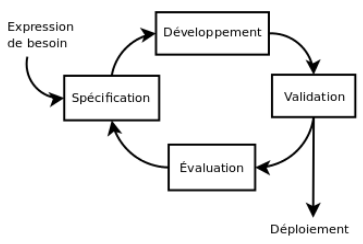
\includegraphics[scale=0.8]{\images/cycleiteratif.png}
                \caption{Le processus du cycle itératif}
            \end{figure}
           
            \vspace{0.2cm}

            Cette méthode présente 6 étapes marquante : 
            \begin{itemize}
                \renewcommand{\labelitemi}{$\bullet$}
                \item L’expression de besoin: où les exigences sont mis en place. L’idée reste que 
                les informations en entrée peuvent être modifiées par la suite du processus itératif.\\
                Le cercle du processus itératif: 
                \begin{itemize}
                    \renewcommand{\labelitemi}{$\bullet$}
                    \item  La spécification technique du besoin 
                    \item  Le développement : la période où on implémente la spec
                    \item  La validation : une étape qui est marqué par les tests.C’est l’ensemble des tests qui 
                    permettent de s’assurer que le développement effectué correspond bien à ce qui était attendu.
                    \item  L’évaluation : Cette étape sert à effectuer un retour sur les fonctionnalités laissés. 
                    Ceci sert comme des informations d’entrée pour un nouveau cycle.
                \end{itemize} 
                \item Déploiement : l’étape finale qui consiste à ce que les livrables validés sont livrés.  
            \end{itemize}

             \vspace{0.5cm}
            
            Ce type de cycle de développement est le plus souple des méthodologies:
             chaque itération permet de s’adapter à ce qui a été appris dans les itérations précédentes et 
             le projet fini peut varier du besoin qui a été exprimé à l’origine.\cite{cycle_iteratif} \\
            
            Vu la nature du projet qui part plutôt vers une étude de faisabilité avec des critères de performances, 
            l’expression des besoins peuvent être redéfinies pendant ce temps. Il est préférable de suivre une méthodologie 
            souple d’où le choix de telle méthodologie. 
            


        \subsubsection{MD30 est un travail d'équipe suivi}

        le projet MD30 présente le nouveau protocole de communication entre les boîtiers OBD et le CLoud et donc le projet 
        invoque les boîtiers ainsi que le point d entrée du cloud. \\ [0.3cm]
        Le projet MD30 engage 5 personnes dans deux différentes parties : 
        \begin{itemize}
            \renewcommand{\labelitemi}{$\bullet$}
            \item 2 personnes sur MD30 côté Serveur
            \item 3personnes sur MD30 côté Core
        \end{itemize} 
         
        \vspace{0.2cm}
        
        Même si le coeur de développement des deux parties est totalement indépendant l’un de l'autre. Les deux parties doivent 
        rester synchroniser sur l'avancement de chaque partie afin d'avancer dans le projet en phase. C'est pour cela qu'une réunion  
        hebdomadaire de synchronisation s'effectue chaque fin de semaine. 
        Le suivi de ce projet se fait à travers la création des ticket en utilisant l'outil Asana.\\

        Asana est un outil de gestion de projet web et mobile qui donne une visibilité sur  ..... 
        

        figure : What asana dashboard looks like 